\head{Февраль}{Листок Весёлый.}

\textit{Для поднятия настроения и «боевого духа» в качестве бонуса для тех, кто раньше всех успешно
справился с предыдущим листком.}

\begin{thmF}
    Однажды король призвал ко двору четырёх великих мудрецов. Он собрал их всех в своём тронном зале и показал им 7 золотых табличек. На первой было написано число 1, на второй 2, ..., на седьмой 7. Затем он объявил мудрецам, что каждый из них получит одну из этих табличек. После чего он перемешал таблички и дал каждому мудрецу по одной. Таким образом, каждый мудрец знал, какое число досталось ему, но не знал, какие числа достались другим. Раздав таблички, король спросил первого мудреца: 
    \par -- Твоё число больше чем числа других мудрецов?
    \par -- Я не знаю, -- ответил первый мудрец. 
    \\ Затем король спросил второго мудреца: 
    \par -- Твоё число больше, чем числа других мудрецов?
    \par -- Я не знаю, -- ответил второй мудрец.
    \\ Король спросил третьего мудреца: 
    \par -- Твоё число больше, чем числа других мудрецов? 
    \par -- Я не знаю, -- ответил третий мудрец.
    \\ Наконец спросил король четвёртого мудреца: 
    \par -- Твоё число больше чем числа других мудрецов?
    \par -- Да, -- ответил тот. 
    \par -- Ты уверен в этом? -- переспросил его король. 
    \par -- Совершенно уверен. Более того, про каждого из мудрецов я точно знаю, какое число ему досталось.
    \\ Подивился король уму своих мудрецов, однако нас их ответы не должны удивлять. Определите про каждого из мудрецов, какое число ему досталось. 
\end{thmF}
{\footnotesize \textit{(Важное пояснение к задаче: про каждого из мудрецов общеизвестным является то, что он обладает совершенным интеллектом, то есть мгновенно может из имеющейся у него информации сделать все логические выводы)}}

\begin{figure}[h]
    \begin{minipage}{0.75\linewidth}
        \begin{thmF}
            Маша положила на стол несколько отрезков и обнаружила четыре квадрата, все стороны которых лежат на этих отрезках. Все четыре квадрата были разных размеров. (Пример такого расположения отрезков показан на рисунке.) Докажите, что Маша может переложить отрезки так, чтобы квадратов оказалось шесть (и все разных размеров).
        \end{thmF}
    \end{minipage}
\hfill
    \begin{minipage}{0.2\linewidth}
        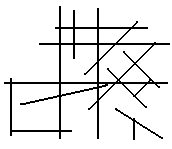
\includegraphics[width=0.95\columnwidth]{img/10.8.0 img1.png}
    \end{minipage}
\end{figure}

\begin{thmF}
    На выборах в Стране Чудаков можно было проголосовать за партию жуликов, партию воров или партию дураков (за какую--то одну). Всего бюллетеней было столько же, сколько избирателей, но некоторые избиратели не пришли, и их бюллетени оказались незаполненными. Тогда партия воров украла половину этих бюллетеней и заполнила в свою пользу. После этого при подсчёте голосов партии жуликов удалось присвоить треть голосов за каждую из остальных партий. В результате партия дураков набрала 25\% (от числа заполненных бюллетеней). Если бы выборы были честными, партия дураков набрала бы более 50\% от числа заполненных бюллетеней. Докажите, что явка на выборы была не более 60\%, если известно, что все бюллетени были заполнены правильно.
\end{thmF}